
\begin{frame}{Has someone done this before?}
  \cite{Wojek_etal_2013} \\
  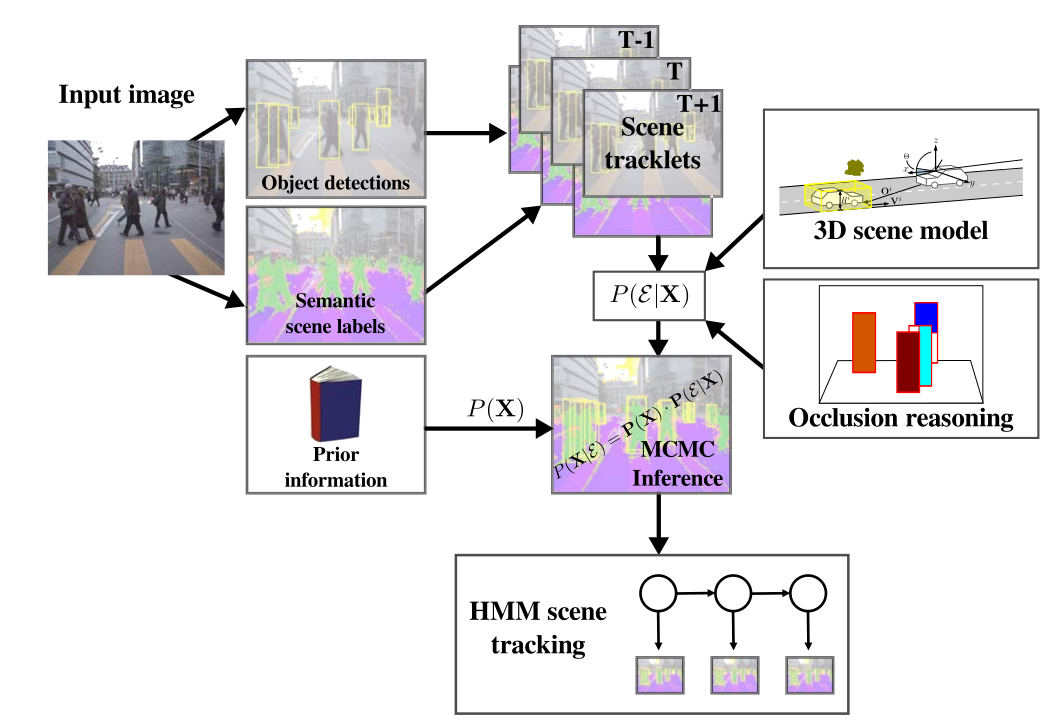
\includegraphics[width=0.8\textwidth]{graphics/wojek2013.png}
  % did exactly same way but we have better occlusion model because our
  % occlusion models are continous.
    
\end{frame}

\begin{frame}{\cite{Geiger_etal_2012} }
  % used stereo imagery and a restricted lane model that
  % reduce vehicle localization to a 1-D search on the lane.
  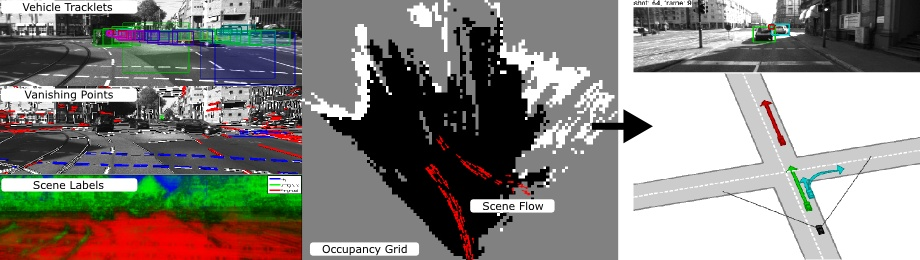
\includegraphics[width=\textwidth]{graphics/geiger_intersection_2012_1.jpg}\\
  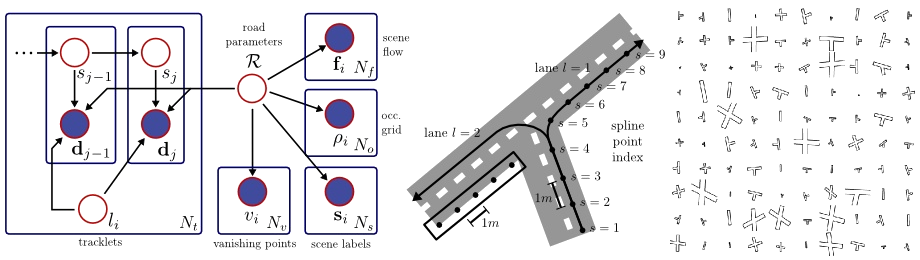
\includegraphics[width=\textwidth]{graphics/geiger_intersection_2012_2.png}
    
\end{frame}

\begin{frame}{ \cite{Milan_etal_2014}}
  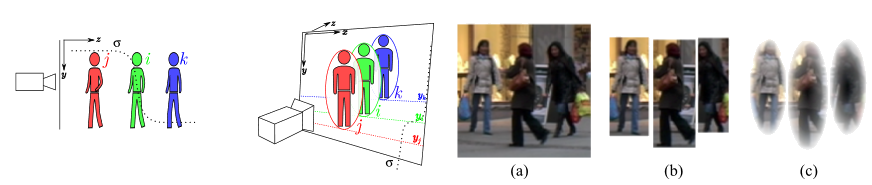
\includegraphics[width=\textwidth]{graphics/milan2014.png}
  % Use continuous occlusion model in multi-tracking framework but those are
  % just in 2D, our occlusion model is more principled and is in 3D.
    
\end{frame}

\begin{frame}{What is missing?}
  \begin{itemize}
    \item Traffic-Scene interaction
    \item Traffic traffic interaction
  \end{itemize}
\end{frame}

